\section{Diverses}
\subsection{Physikalische Zuordnung logischer Zustände}
\begin{flushleft}
    \begin{tabular}{c l l}
        $0$ & Low \SI{0}{\volt} & Ground\\
        $1$ & High \SI{0.8}{\volt} & VDD
    \end{tabular}
\end{flushleft}
Toleranzen:
\begin{itemize}
    \item GND: \SIrange{0}{0.15}{\volt}
    \item VDD \SIrange{0.7}{0.9}{\volt}
\end{itemize}
\subsection{Schaltelemente}
\begin{center}
    \begin{minipage}[t]{0.45\linewidth}
        \subsubsection{Multiplexer}
        Sendet eines von $2^n$ Eingangssignalen an den Ausgang. Hat $n$ Auswahlbits.
    \end{minipage}
    \hfill
    \begin{minipage}[t]{0.45\linewidth}
        \subsubsection{Demultiplexer}
        Sendet $1$ Eingangssignal an einen von $2^n$ Ausgänge. $n$ Auswahlbits.
    \end{minipage}
\end{center}
\subsubsection{Halbaddierer}
Addiert 2 Binärzahlen $A$ und $B$. Produziert Summe und Carry-Out.
\begin{equation*}
    \text{SUM} = A \oplus B \qquad \text{CO} = A \land B
\end{equation*}
\subsubsection{Volladdierer}
Nimmt einen zusätzlichen Input $CI$ entgegen.
\begin{equation*}
    \text{SUM} = (A \oplus B) \oplus CI \qquad \text{CO} = (A \land B) \lor (S_{AB} \land CI) 
\end{equation*}

\subsubsection{Serienaddierer}
Addition \underline{einer} Stelle pro Taktschritt.

\subsubsection{Paralleladdierer (Normalform)}
Addition \underline{aller} Stellen pro Taktschritt.
\begin{center}
    \small
    \begin{minipage}[t]{0.45\linewidth}
        \paragraph{Vorteile}
        \begin{itemize}
            \item Maximal 3 Grundgatter zwischen Input und Output.
            \item Laufzeit ist unabhängig von Stellenzahl der Summanden.
        \end{itemize}
    \end{minipage}
    \hfill
    \begin{minipage}[t]{0.45\linewidth}
        \paragraph{Nachteile}
            Bei Addition von $n$-stelligen Summanden müssen $\sim n \cdot 2^{2n - 1}$ Min-/Maxterme verknüpft werden.
    \end{minipage}
\end{center}
$\rightarrow$ Schnell aber Schaltungsaufwendig

\subsubsection{Ripple-Carry Addierer (Paralleladdierer)}
\begin{center}
    \small
    \begin{minipage}[t]{0.45\linewidth}
        \paragraph{Vorteile}
        \begin{itemize}
            \item Durch Kaskadierung einfach skalierbar.
            \item Schaltungsaufwand linear zur Stellenzahl.
        \end{itemize}
    \end{minipage}
    \hfill
    \begin{minipage}[t]{0.45\linewidth}
        \paragraph{Nachteile}
        \begin{itemize}
            \item SUM und CO für die $i$-te Stelle können erst nach der Berechnung der $(i-1)$-ten Stelle gebildet werden.
            \item Addierzeit linear zu Stellenzahl
        \end{itemize}
    \end{minipage}
\end{center}
Langsamer als Normalformaddierer aber einfacher zu realisieren.

\subsubsection{Carry-Look-Ahead Addierer (Paralleladdierer)}
Kombination der Vorteile des Normalform- und Ripple-Carry-Addierer $\rightarrow$ schnelle Schaltung mit begrenztem Aufwand.
\paragraph{Praktische Realisierung} Addierer werden kaskadiert, Berechnung der Überträge erfolgt parallel zur Summenbildung.\\
Berechnungsaufwand ist linear zur Stellenzahl, Laufzeit bleibt konstant.

\subsection{Booth-Algorithmus}
Dient der Multiplikation von Binärzahlen ($A$ \& $B$).\\
Berechnung über Zwischenprodukte $P_i$.\\
Division durch 2 bedeutet: Verschiebung des Kommas nach links (shift), mit Vorzeichenverdoppelung falls nötig.
\begin{center}
    \begin{tabular}{c c l}
        $a_i$ & $a_{i - 1}$ & Operation\\
        \hline
        $0$ & $0$ & $P_i = P_{i-1}/2$\\
        $0$ & $1$ & $P_i = (P_{i-1} + B)/2$\\
        $1$ & $0$ & $P_i = (P_{i-1} - B)/2$\\
        $1$ & $1$ & $P_i = P_{i-1}/2$\\
    \end{tabular}
\end{center}
Anfangswerte: $P_{-1} = 0$, $a_{-1} = 0$\\
Beim letzten Schritt entfällt die Division durch 2.

\subsection{Zahlencodes}
\begin{center}
    \csvreader[
        separator=semicolon,
        tabular=|c|cccccc|,
        head=true,
        table head=\hline\rotatebox{90}{Binär} & \rotatebox{90}{BCD} & \rotatebox{90}{Excess-3~} & \rotatebox{90}{Aiken} & \rotatebox{90}{4-2-2-1} & \rotatebox{90}{Gray} & \rotatebox{90}{O'Brien}\\\hline,
        table foot = \hline,
        late after line=\csvifoddrow{\\\rowcolor{white}}{\\\rowcolor{primaryheader!15}}
        ]{tables/codes.csv}{
            1=\binary, 
            2=\bcd, 
            3=\excessThree, 
            4=\aiken, 
            5=\ftto, 
            6=\gray, 
            7=\obrien
            }{%
            \binary & \bcd & \excessThree & \aiken & \ftto & \gray & \obrien
    }%
\end{center}

\subsection{Gate Varianten}
\begin{center}
    \rotatebox{90}{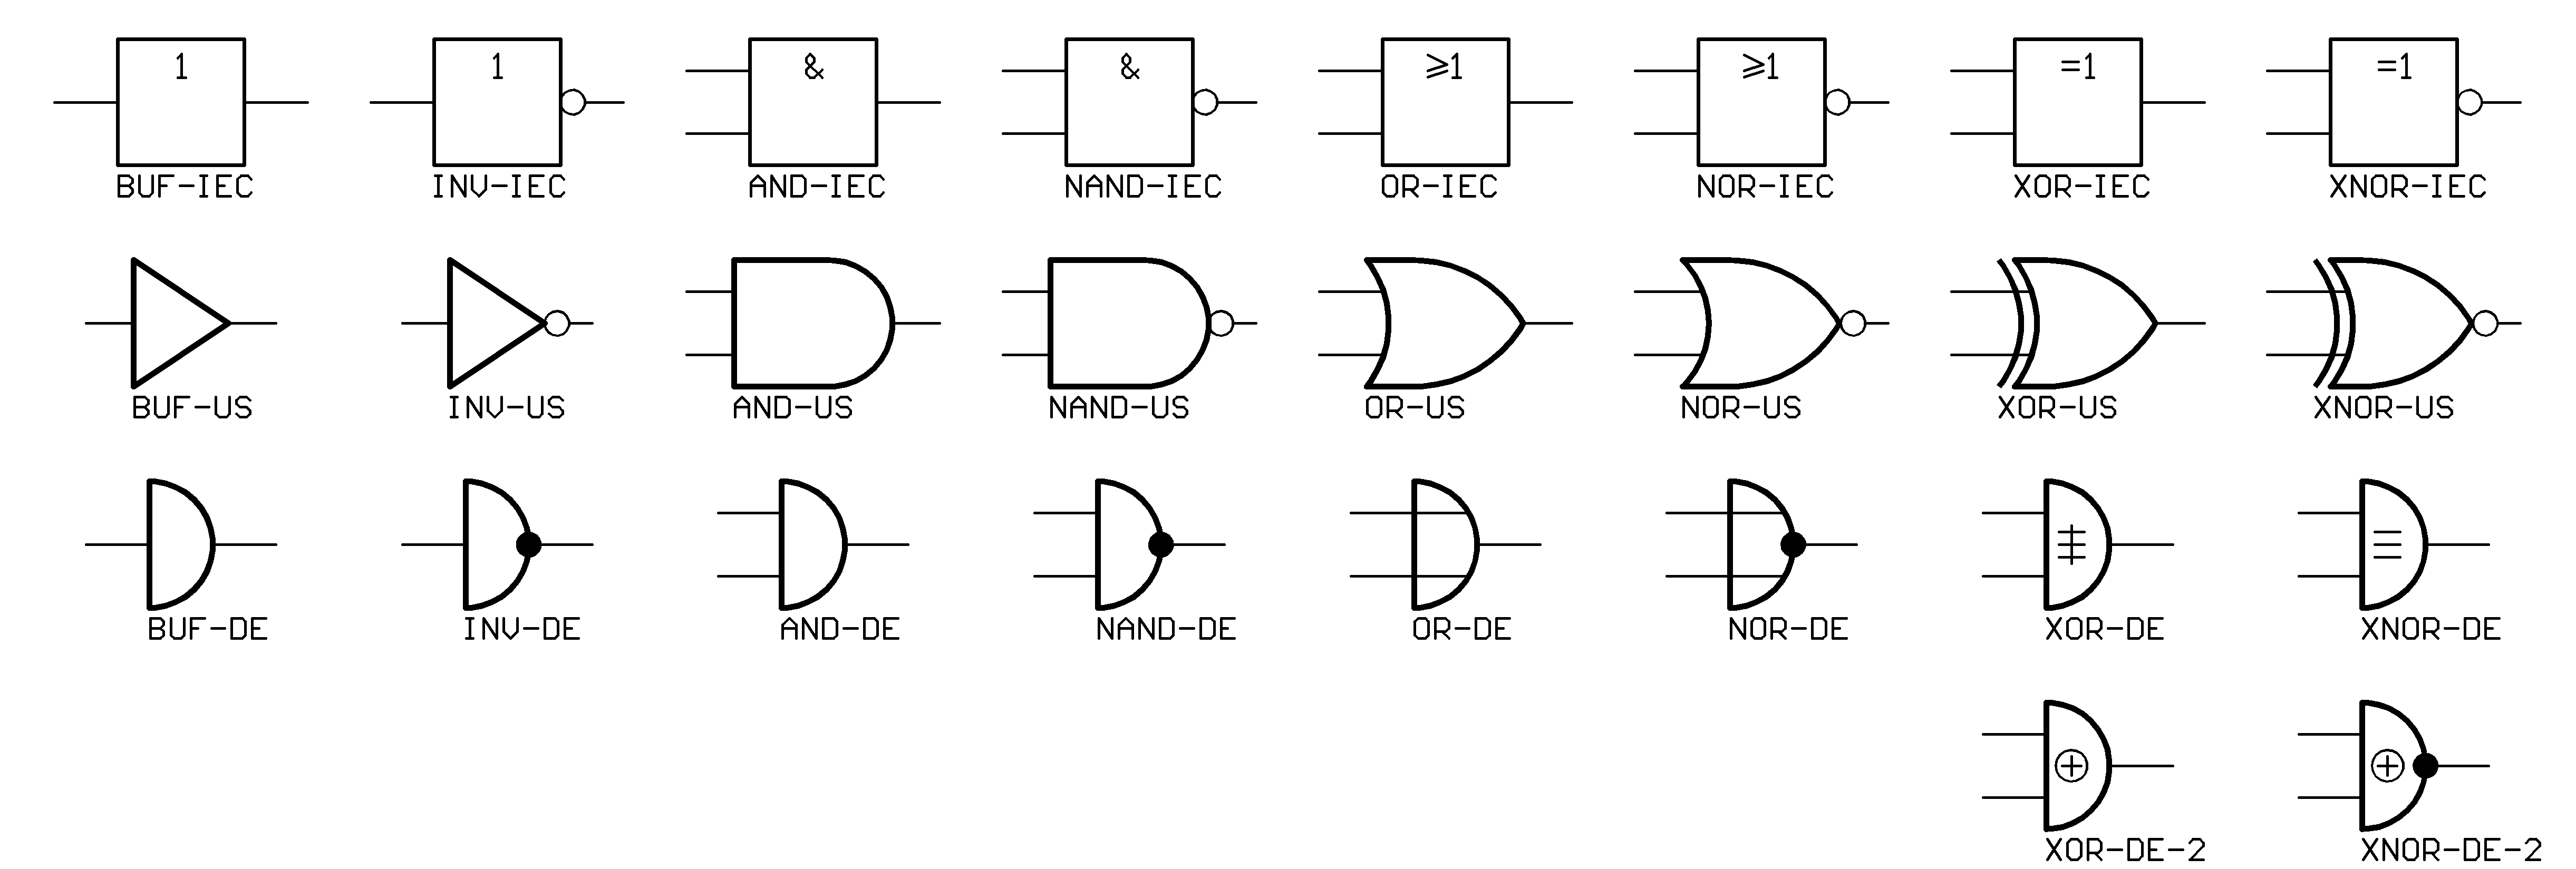
\includegraphics[height = 50mm]{images/Logic-gate-index.png}}
\end{center}